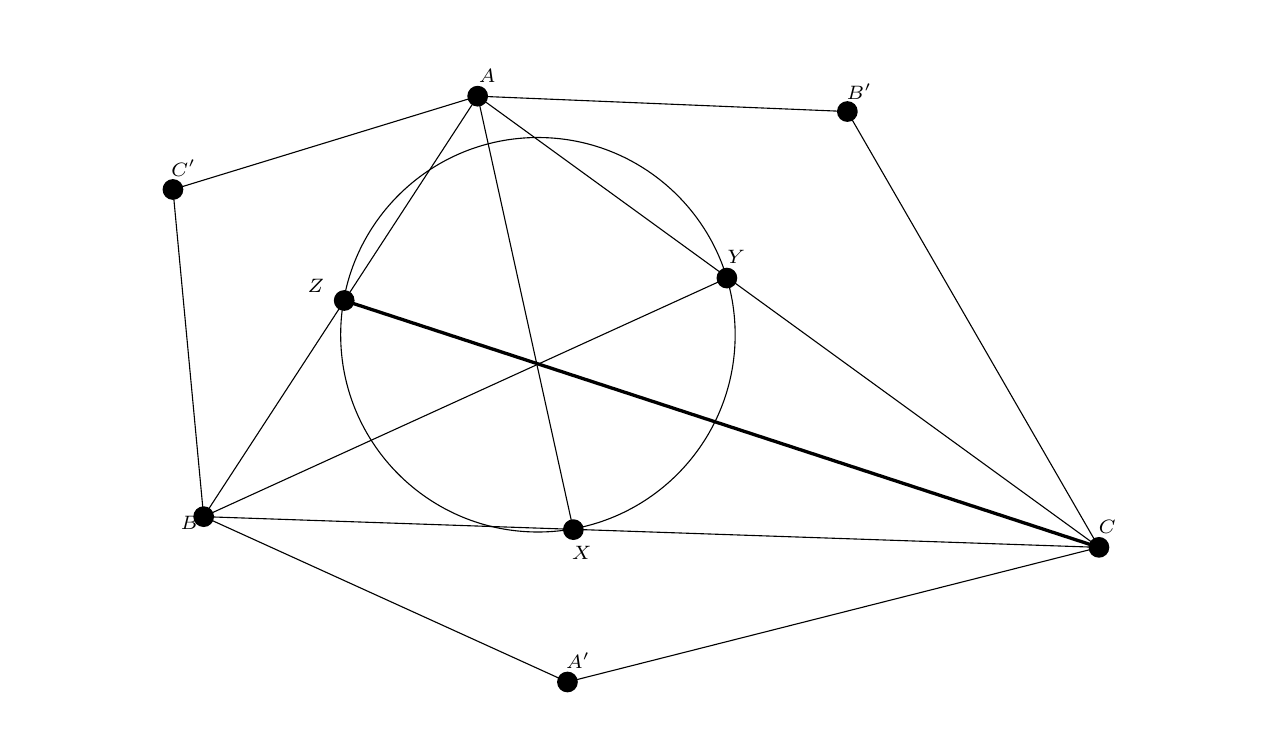
\begin{tikzpicture}[line cap=round,line join=round,xscale=1.5,yscale=1.5]
    \clip(-0.05,-1.59) rectangle (10.32,4.34);
    \draw (3.76,3.76)-- (1.44,0.2);
    \draw (1.44,0.2)-- (9.02,-0.06);
    \draw (9.02,-0.06)-- (3.76,3.76);
    \draw (3.76,3.76)-- (1.18,2.97);
    \draw (1.18,2.97)-- (1.44,0.2);
    \draw (1.44,0.2)-- (4.52,-1.2);
    \draw (4.52,-1.2)-- (9.02,-0.06);
    \draw (9.02,-0.06)-- (6.89,3.63);
    \draw (6.89,3.63)-- (3.76,3.76);
    \draw (3.76,3.76)-- (4.57,0.09);
    \draw (1.44,0.2)-- (5.87,2.22);
    \draw(4.27,1.74) circle (1.67cm);
    \draw [line width=1.2pt] (9.02,-0.06)-- (2.63,2.03);
    \begin{scriptsize}
        \fill [color=black] (3.76,3.76) circle (2.5pt);
        \draw[color=black] (3.84,3.93) node {$A$};
        \fill [color=black] (1.44,0.2) circle (2.5pt);
        \draw[color=black] (1.32,0.15) node {$B$};
        \fill [color=black] (9.02,-0.06) circle (2.5pt);
        \draw[color=black] (9.09,0.11) node {$C$};
        \fill [color=black] (4.52,-1.2) circle (2.5pt);
        \draw[color=black] (4.61,-1.02) node {$A'$};
        \fill [color=black] (6.89,3.63) circle (2.5pt);
        \draw[color=black] (6.99,3.8) node {$B'$};
        \fill [color=black] (1.18,2.97) circle (2.5pt);
        \draw[color=black] (1.27,3.15) node {$C'$};
        \fill [color=black] (4.57,0.09) circle (2.5pt);
        \draw[color=black] (4.64,-0.11) node {$X$};
        \fill [color=black] (5.87,2.22) circle (2.5pt);
        \draw[color=black] (5.95,2.4) node {$Y$};
        \fill [color=black] (2.63,2.03) circle (2.5pt);
        \draw[color=black] (2.39,2.15) node {$Z$};
    \end{scriptsize}
\end{tikzpicture}
